% Underlying graph for minimum spanning tree (mst) example
% Redrawn from Figure 5.3 of the textbook ``Algorithms'' by Dasgupta

\documentclass{standalone}

\usepackage{tikz}
\usetikzlibrary{mindmap, positioning, backgrounds, fit}

\begin{document}
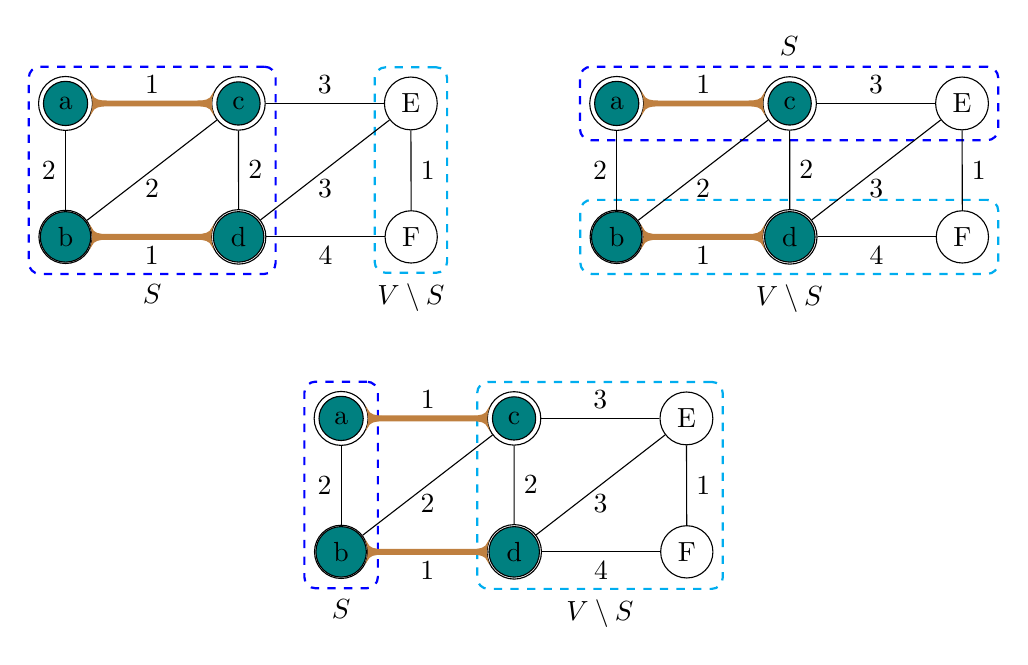
\begin{tikzpicture}[node distance = {1.0cm and 1.5cm}, 
	v/.style = {draw, circle},
    cpv/.style = {v, fill = teal},	% vertices in cut property example
    cpe/.style = {circle connection bar, brown, fill}, % edges in cut property example
	cut/.style = {rectangle, rounded corners, dashed, draw, thick}	% cut
	]
  \begin{scope}
	\node (a) [v] {A};
	\node (c) [v, right = of a] {C};
	\node (e) [v, right = of c] {E};
	\node (b) [v, below = of a] {B};
	\node (d) [v, right = of b] {D};
	\node (f) [v, right = of d] {F};

	% edges
    \draw (a) to node[above] {1} (c);
    \draw (c) to node[above] {3} (e);
    \draw (b) to node[below] {1} (d);
    \draw (d) to node[below] {4} (f);
    \draw (a) to node[left] {2} (b);
    \draw (c) to node[below] {2} (b);
    \draw (c) to node[right] {2} (d);
    \draw (e) to node[below] {3} (d);
    \draw (e) to node[right] {1} (f);

	% edges X
	\foreach \v in {a, b, c, d}{
	  \node[cpv] at (\v) {\MakeUppercase{\v}};
	}
	\draw[cpe] (a) to (c);
	\draw[cpe] (b) to (d);

	% cut 1 (respecting X)
	\begin{pgfonlayer}{background}
	  \node () [cut, blue, fit = (a) (b) (c) (d), label = {below:$S$}] {};
	  \node () [cut, cyan, fit = (e) (f), label = {below:$V \setminus S$}] {};
	\end{pgfonlayer}
  \end{scope}

  % cut 2 (respecting X)
  \begin{scope}[xshift = 7.0cm]
	% the nodes
	\node (a) [v] {A};
	\node (c) [v, right = of a] {C};
	\node (e) [v, right = of c] {E};
	\node (b) [v, below = of a] {B};
	\node (d) [v, right = of b] {D};
	\node (f) [v, right = of d] {F};

	% edges
    \draw (a) to node[above] {1} (c);
    \draw (c) to node[above] {3} (e);
    \draw (b) to node[below] {1} (d);
    \draw (d) to node[below] {4} (f);
    \draw (a) to node[left] {2} (b);
    \draw (c) to node[below] {2} (b);
    \draw (c) to node[right] {2} (d);
    \draw (e) to node[below] {3} (d);
    \draw (e) to node[right] {1} (f);
	
    % edges X
	\foreach \v in {a, b, c, d}{
	  \node[cpv] at (\v) {\MakeUppercase{\v}};
	}
    \draw[cpe] (a) to (c);
    \draw[cpe] (b) to (d);

	\begin{pgfonlayer}{background}
	  \node () [cut, blue, fit = (a) (c) (e), label = {above:$S$}] {};
	  \node () [cut, cyan, fit = (b) (d) (f), label = {below:$V \setminus S$}] {};
	\end{pgfonlayer}
  \end{scope}

  % cut 3 (not respect X)
  \begin{scope}[xshift = 3.5cm, yshift = -4.0cm]
	% the nodes
	\node (a) [v] {A};
	\node (c) [v, right = of a] {C};
	\node (e) [v, right = of c] {E};
	\node (b) [v, below = of a] {B};
	\node (d) [v, right = of b] {D};
	\node (f) [v, right = of d] {F};

	% edges
    \draw (a) to node[above] {1} (c);
    \draw (c) to node[above] {3} (e);
    \draw (b) to node[below] {1} (d);
    \draw (d) to node[below] {4} (f);
    \draw (a) to node[left] {2} (b);
    \draw (c) to node[below] {2} (b);
    \draw (c) to node[right] {2} (d);
    \draw (e) to node[below] {3} (d);
    \draw (e) to node[right] {1} (f);

    % edges X
	\foreach \v in {a, b, c, d}{
	  \node[cpv] at (\v) {\MakeUppercase{\v}};
	}
    \draw[cpe] (a) to (c);
    \draw[cpe] (b) to (d);

	\begin{pgfonlayer}{background}
	  \node () [cut, blue, fit = (a) (b), label = {below:$S$}] {};
	  \node () [cut, cyan, fit = (c) (d) (e) (f), label = {below:$V \setminus S$}] {};
	\end{pgfonlayer}
  \end{scope}
\end{tikzpicture}
\end{document}